\documentclass[12pt, notitlepage]{article}
\usepackage[margin=1in, top=0.5in]{geometry}
\usepackage[utf8x]{inputenc}
\usepackage{gensymb}
\usepackage{array}
\usepackage{amssymb}
\usepackage{amsmath}
\usepackage{graphicx}
\usepackage{tabularx}
\usepackage{pbox}
\usepackage[makeroom]{cancel}
\usepackage{float}
\usepackage{caption}
\usepackage{newfloat}
\DeclareFloatingEnvironment[name={Gráfico}]{graph}
\newcommand\numberthis{\addtocounter{equation}{1}\tag{\theequation}}
\setcounter{MaxMatrixCols}{20}


\title{Título}

\date{\today}
\renewcommand{\contentsname}{Contenidos}
\renewcommand\refname{Referencias}
\renewcommand\tablename{Tabla}
\renewcommand\figurename{Figura}
\newcommand{\norm}[1]{\left\lVert#1\right\rVert}

\geometry{letterpaper}

\begin{document}
\thispagestyle{empty}
\setlength{\unitlength}{1 cm} %Especificar unidad de trabajo
\begin{picture}(18,4)
\put(0,0){
\includegraphics[scale=0.38]{UTFSM_logo.png}}
\put(11.5,0){
\includegraphics[scale=0.2]{mecusm.jpg}}
\end{picture}
\\
\\
\begin{center}
{\LARGE {Universidad Técnica Federico Santa María}}\\[0.5cm]
{\Large Departamento de Ingeniería Mecánica}\\[2cm]
%{\Large Redes}\\[2.3cm]
{\Huge \textbf{Tarea 5:}}\\[0.2cm]
{\Huge \textbf{``Método de diferencias finitas aplicado a transferencia de calor en una placa"}}\\[0.2cm]
{\large IPM-458 - Computación Científica.}\\[3cm]
{\large Alumno: Nicolás Espinoza M.}\\[3cm]
Profesor: Franco Perazzo M.\\
Ayudante: Luis Fuenzalida L.\\[3cm]
Valparaíso - Julio 05, 2017
\end{center}
\newpage
\tableofcontents
\newpage

\section{Presentación del problema}
El presente informe desarrolla el método de diferencias finitas, en particular de segundo orden, aplicado a la transferencia de calor en una placa cuadrada. La placa tiene dos tipos de condiciones:
\begin{itemize}
\item{Dirichlet en los bordes superior y derecho.}
\item{Neumann en los bordes inferior e izquierdo.}
\end{itemize}

Los valores de estas condiciones se pueden ver en la Figura 1. Se consideran dos dimensiones (ejes $x$ e $y$), con un mismo número $n$ de nodos en ambas direcciones. La ecuación que rige el problema planteado, transferencia de calor en dos dimensiones en estado estacionario, es
\begin{equation}
\frac{\partial^2T(\vec{x})}{\partial x^2} + \frac{\partial^2T(\vec{x})}{\partial y^2} = 0
\end{equation}

Discretizando con diferencias finitas centradas (2\degree orden), obtenemos la aproximación siguiente:

\begin{equation}
\frac{\partial^2T(\vec{x})}{\partial x^2} + \frac{\partial^2T(\vec{x})}{\partial y^2} \approx \frac{T_{i+1,j} - 2T_{i,j} + T_{i-1,j}}{(\Delta x)^2} + \frac{T_{i,j+1} - 2T_{i,j} + T_{i,j-1}}{(\Delta y)^2} = 0
\end{equation}

Esta ecuación es la que se utilizará para aproximar las soluciones del sistema, a modo de trabajar con resultados numéricos y poder programar la situación en el computador. Como los pasos en ambas direcciones tienen el mismo tamaño, se puede trabajar con la ecuación simplificada siguiente, en remplazo de la Ecuación 2:

\begin{equation}
T_{i+1,j} + T_{i-1,j} - 4T_{i,j} + T_{i,j+1} + T_{i,j-1} = 0
\end{equation}

\begin{figure}[H]
\centering
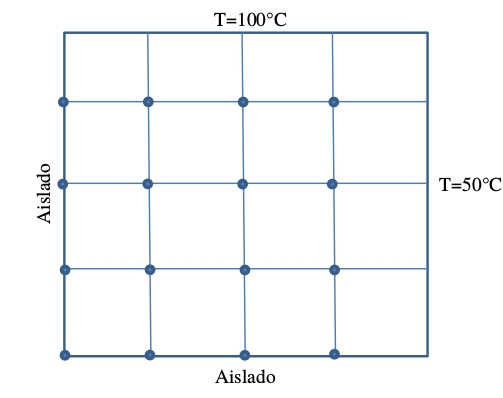
\includegraphics[scale=0.6]{Esquema.jpg}
\caption{Discretización de la placa mediante el método de diferencias finitas de segundo orden.}
\end{figure}

\section{Establecimiento de las ecuaciones para los distintos tipos de nodo}
En esta placa se tienen distintos tipos de condiciones, por lo que se tienen distintas ecuaciones para los diferentes tipos de nodo. En esta sección se establecerán dichas ecuaciones según dónde se ubican los nodos a tratar.

\subsection{Nodos del borde izquierdo}
Para estos nodos, la condición que se cumple es la de Neumann. Las paredes están aisladas, por lo que la condición queda igualada a cero.

\begin{gather*}
-k\left.\frac{\partial T}{\partial x}\right|_{x = 0} = \dot{q} = 0 \\
\frac{T_{i+1,j} - T_{i-1,j}}{2\Delta x} = 0 \rightarrow T_{i+1,j} = T_{i-1,j}\\
2T_{i+1,j} - 4T_{i,j} + T_{i,j+1} + T_{i,j-1} = 0
\end{gather*}

La $3^a$ ecuación es la que modela la transferencia con diferencias finitas, habiendo remplazado la condición de Neumann correspondiente.

\subsection{Nodos del borde inferior}
Se cumple la misma condición en los nodos inferiores, pero la diferencia es que se considera la coordenada $y$ en vez de la $x$. Luego, las condiciones de contorno y la ecuación para este tipo de nodos es:

\begin{gather*}
-k\left.\frac{\partial T}{\partial y}\right|_{y = 0} = \dot{q} = 0 \\
\frac{T_{i,j+1} - T_{i,j-1}}{2\Delta y} = 0 \quad \longrightarrow\quad T_{i,j+1} = T_{i,j-1}\\
T_{i+1,j} + T_{i-1,j} - 4T_{i,j} + 2T_{i,j+1} = 0
\end{gather*}

\subsection{Esquina inferior izquierda}
El nodo de la esquina inferior izquierda está aislado por abajo y por la izquierda, por lo que se aplican las dos condiciones anteriores simultáneamente:

\begin{equation*}
2T_{i+1,j} - 4T_{i,j} + 2T_{i,j+1} = 0
\end{equation*}

\subsection{Nodos del borde superior}
Los nodos en este borde tienen una temperatura dada, lo que corresponde a una condición de tipo Dirichlet. La ecuación en este caso queda como

\begin{align*}
T_{i,j} = T_{borde}&\\
\text{En este caso, corresponde a}\ T_{i,j} &= 100\degree C
\end{align*}

Para los nodos inmediatamente inferiores a estos sin embargo, nos sirve esta condición, pues se despeja la temperatura conocida $T_{i,j+1} = 100$ como solución de la ecuación, quedando para los nodos $j=n-1$:

\begin{equation*}
-4T_{i,j} + T_{i+1,j} + T_{i-1,j} + T_{i,j-1} = -100
\end{equation*}

\subsection{Nodos en el borde derecho}
Para el borde derecho se repite la situación de los nodos en el borde superior, pero en la otra dirección y con otro valor de $T_{borde}$.

\begin{gather*}
T_{i,j} = T_{borde} \\
T_{borde} = 50\degree C
\end{gather*}

Nuevamente, para los nodos directamente a la izquierda de los del borde, nos resulta útil esta condición, pues permite utilizar esa condición de Dirichlet como resultado de las ecuaciones que modelan a aquellos.

\begin{equation*}
-4T_{i,j} + T_{i-1,j} + T_{i,j+1} + T_{i,j-1} = -50
\end{equation*}

\subsection{Esquina superior derecha i = n-1, j = n-1}
Esta esquina tiene dos condiciones de Dirichlet asociadas, que son las temperaturas de los bordes derecho y superior. La ecuación de este nodo queda así:
\begin{equation}
-4T_{i,j} + T_{i-1,j} + T_{i,j-1} = -150
\end{equation}

\subsection{Nodos interiores}
Estos nodos, que no están en el borde sino que en el centro, tienen otro nodo como vecino en ambas direcciones en ambos ejes. La Ecuación 3 se mantiene para este tipo de nodos, sin cambio.\\\\
El siguiente paso es establecer la matriz de factores y el vector de resultados, y programar o aplicar el método de resolución del sistema.

\subsection{Matriz de cofactores}
La matriz de cofactores A del sistema en el caso de paso $\Delta = 12.5 [cm]$ es la siguiente

\begin{equation*}
\begin{pmatrix}
-4. &  2. &  0. &  0. &  1. &  0. &  0. &  0. &  0. &  0. &  0. &  0. &  0. &  0. &  0. &  0. \\
 1. & -4. &  1. &  0. &  0. &  1. &  0. &  0. &  0. &  0. &  0. &  0. &  0. &  0. &  0. &  0. \\
 0. &  1. & -4. &  1. &  0. &  0. &  1. &  0. &  0. &  0. &  0. &  0. &  0. &  0. &  0. &  0. \\
 0. &  0. &  1. & -4. &  0. &  0. &  0. &  1. &  0. &  0. &  0. &  0. &  0. &  0. &  0. &  0. \\
 1. &  0. &  0. &  0. & -4. &  2. &  0. &  0. &  1. &  0. &  0. &  0. &  0. &  0. &  0. &  0. \\
 0. &  1. &  0. &  0. &  1. & -4. &  1. &  0. &  0. &  1. &  0. &  0. &  0. &  0. &  0. &  0. \\
 0. &  0. &  1. &  0. &  0. &  1. & -4. &  1. &  0. &  0. &  1. &  0. &  0. &  0. &  0. &  0. \\
 0. &  0. &  0. &  1. &  0. &  0. &  1. & -4. &  0. &  0. &  0. &  1. &  0. &  0. &  0. &  0. \\
 0. &  0. &  0. &  0. &  1. &  0. &  0. &  0. & -4. &  2. &  0. &  0. &  1. &  0. &  0. &  0. \\
 0. &  0. &  0. &  0. &  0. &  1. &  0. &  0. &  1. & -4. &  1. &  0. &  0. &  1. &  0. &  0. \\
 0. &  0. &  0. &  0. &  0. &  0. &  1. &  0. &  0. &  1. & -4. &  1. &  0. &  0. &  1. &  0. \\
 0. &  0. &  0. &  0. &  0. &  0. &  0. &  1. &  0. &  0. &  1. & -4. &  0. &  0. &  0. &  1. \\
 0. &  0. &  0. &  0. &  0. &  0. &  0. &  0. &  2. &  0. &  0. &  0. & -4. &  2. &  0. &  0. \\
 0. &  0. &  0. &  0. &  0. &  0. &  0. &  0. &  0. &  2. &  0. &  0. &  1. & -4. &  1. &  0. \\
 0. &  0. &  0. &  0. &  0. &  0. &  0. &  0. &  0. &  0. &  2. &  0. &  0. &  1. & -4. &  1. \\
 0. &  0. &  0. &  0. &  0. &  0. &  0. &  0. &  0. &  0. &  0. &  2. &  0. &  0. &  1. & -4.
\end{pmatrix}
\end{equation*}
Además, los vectores de incógnitas y solución tienen el orden que se muestra:\\
\begin{gather*}
\text{Vector incógnitas} \qquad \qquad \qquad \qquad \text{Vector solución:}\\
\begin{pmatrix}
T_{1,1}\\
T_{2,1}\\
T_{3,1}\\
T_{4,1}\\
T_{1,2}\\
T_{2,2}\\
T_{3,2}\\
T_{4,2}\\
T_{1,3}\\
T_{2,3}\\
T_{3,3}\\
T_{4,3}\\
T_{1,4}\\
T_{2,4}\\
T_{3,4}\\
T_{4,4}\\
\end{pmatrix} \qquad \qquad \qquad \qquad \qquad \qquad
\begin{pmatrix}
-100\\
-100\\
-100\\
-150\\
0\\
0\\
0\\
-50\\
0\\
0\\
0\\
-50\\
0\\
0\\
0\\
-50\\
\end{pmatrix}
\end{gather*}

\section{Resultados, análisis y conclusiones}
Con este esquema y con el programa en \texttt{Fortran 90} que se adjunta, así como con el método de Gauss-Seidel utilizado en la tarea 2, el sistema tiene la resolución numérica mostrada en los archivos de la siguiente forma:
\begin{itemize}
\item{Temperaturas: Para el caso de n = 4 nodos a resolver, el archivo con las temperaturas es \texttt{output1.txt}. Para n = 8 nodos, el archivo con las temperaturas es \texttt{output2.txt}}
\item{Matriz de Cofactores: Para el caso de n = 4 nodos a resolver, el archivo con los cofactores es \texttt{Mat1.txt}. Para n = 8 nodos, el archivo con la matriz de cofactores es \texttt{Mat2.txt}}
\item{Calores: En este caso el programa devuelve un solo archivo, llamado \texttt{Calor.txt}, en el que se encuentran la componente x del flujo de calor, su componente y, y el módulo. Los valores se encuentran ordenados según la distribución física del problema: El primer elemento de arriba a la izquierda corresponde a la esquina superior izquierda de la placa, por ejemplo.}
\end{itemize}

Los gráficos de Temperaturas y Calores se presentan a continuación:

\begin{figure}[H]
\centering
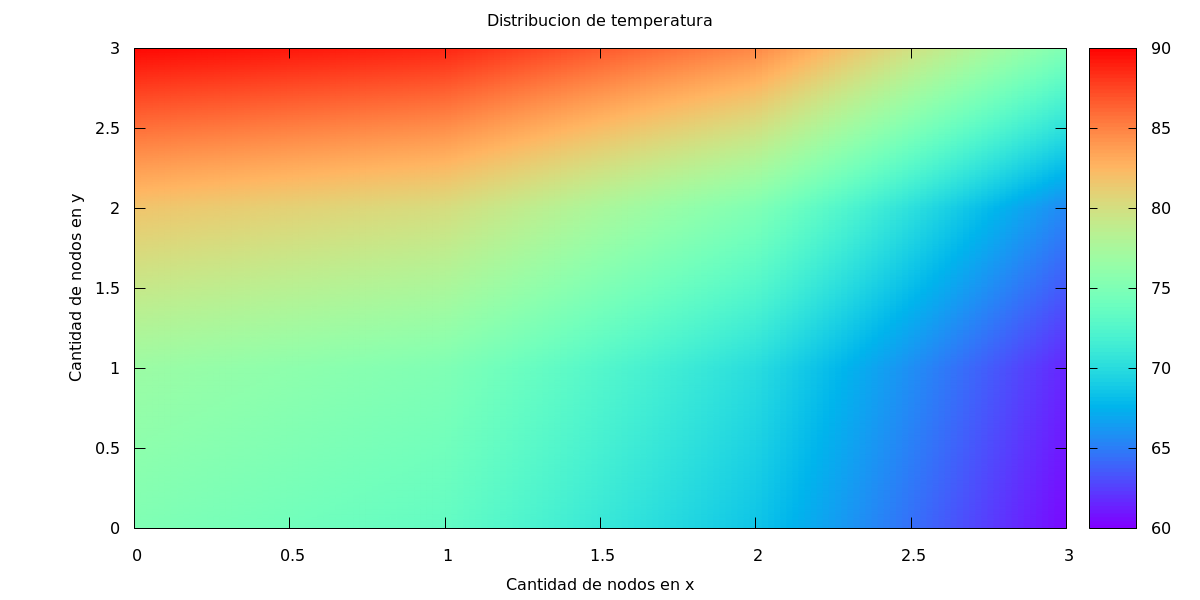
\includegraphics[scale=0.3]{4x4.png}
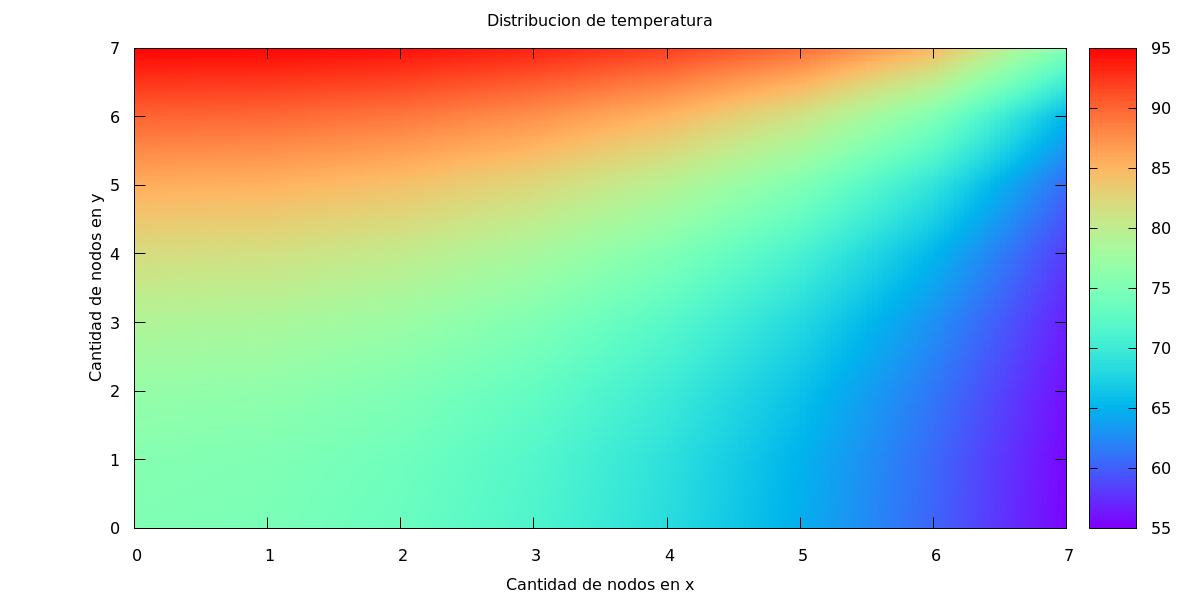
\includegraphics[scale=0.3]{8x8.png}
\caption{Distribución de temperaturas con un sistema 4x4 arriba, y 8x8 abajo.}
\end{figure}

\begin{figure}[H]
\centering
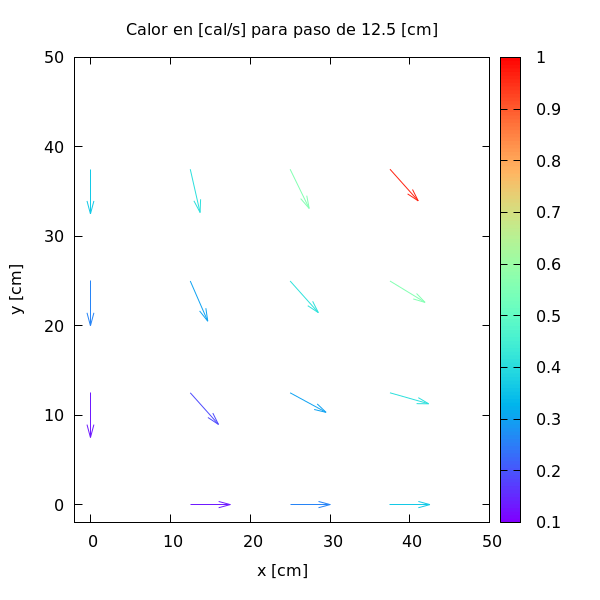
\includegraphics[scale=0.35]{125unit.png}
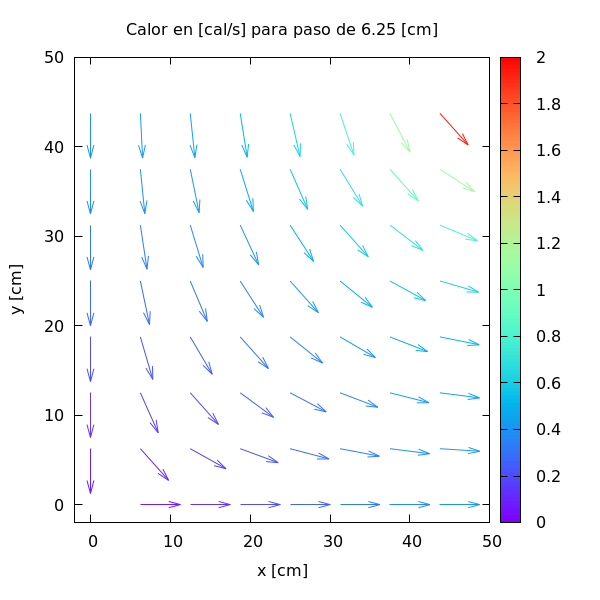
\includegraphics[scale=0.35]{625unit.png}
\caption{Flujos de calor para un sistema 4x4 a la izquierda, y 8x8 a la derecha.}
\end{figure}

Se puede apreciar aquí que los calores fluyen del borde superior de la placa hacia abajo y hacia la izquierda. Esto tiene total sentido físico, pues el lado más frío es el de la derecha, que por termodinámica es el sumidero térmico. Las curvas de temperatura también revelan que como el calor no puede escapar ni por abajo ni por la izquierda, la esquina inferior izquierda recibe calor de arriba y evacúa hacia la derecha.\\\\
El esquema de diferencias finitas es muy útil para aproximar problemas de este estilo, pues sirve muy bien para modelar ecuaciones o sistemas de ecuaciones en derivadas, ya sea parciales u ordinarias. En este caso se resolvió con el método de Gauss-Seidel, que con un error entre iteraciones de $10^{-10}$ nos da una precisión más que suficiente.\\ La transferencia de calor es un ejemplo de esto, pues sin mucha complicación se pudo desarrollar un esquema que generara la matriz de cofactores y que entregara una matriz con las temperaturas en los nodos trabajados. En resumen, diferencias finitas de segundo orden es un método de fácil implementación y con un error de $O(h^2)$, por lo que además tiene una buena precisión y no muy demandante computacionalmente.

\end{document}